
\documentclass{article}
\usepackage{amsmath}
\usepackage{amssymb}
\usepackage{hyperref}
\usepackage{mathrsfs}
\usepackage{enumerate}
\usepackage{bm}
\usepackage{physics}
\usepackage{polynom}
\setlength{\parindent}{0pt}
\usepackage[parfill]{parskip}
\usepackage[margin=1in]{geometry}
\usepackage{tikz}


\begin{document}
\begin{center}
	\huge{\bf Math 100B: Homework 2} \\
	Merrick Qiu
\end{center}

\section*{Problem 1}
We can write $x^{20}+2x^{19} + 5x-7 = (x+2)(x^{19} +5) - 17$
so the remainder is $-17$.
\newpage 

\section*{Problem 2}
The kernel is equal to the ideal 
$\ker \phi = (x^2-4x+5)$
since $x^2-4x+5$ is the monic polynomial of lowest degree
in the kernel.
If there was a polynomial of lower degree 
$ax+b \in \ker \phi$,
then that would imply
$2a +ia + b = 0$ which implies 
$a = 0$ and $b = 0$.
\newpage 

\section*{Problem 3}
The homomorphism
that sends $\tilde{\phi}(x) \to s$
and $\tilde{\phi}(r) \to \phi(r)$ is unique.

The action of this homomorphism on 
a element $\sum a_ix^i \in R[x]$
is uniquely determined by
\[
	\tilde{\phi}\left(\sum a_ix^i\right) =
	\sum \tilde{\phi}(a_i)\tilde{\phi}(x)^i =
	\sum \phi(a_i)s^i.
\]

It is a homomorphism since it sends $1$ to $1$, and it respects
addition and multiplication.
\[
	\tilde{\phi}(1) = \phi(1) = 1
\]

\begin{align*}
	\tilde{\phi}(f+g) &=\tilde{\phi}\left(\sum (a_i+b_i)x^i\right) \\
	&= \sum \tilde{\phi}((a_i+b_i)x^i) \\
	&= \sum \phi(a_i+b_i)s^i \\
	&= \sum \phi(a_i)s^i + \sum \phi(b_i)s^i \\
	&= \tilde{\phi}(f) + \tilde{\phi}(g)
\end{align*}

\begin{align*}
	\tilde{\phi}(fg) &= \tilde{\phi}\left(\sum a_ib_jx^{i+j} \right) \\
	&= \sum \tilde{\phi}\left(\sum a_ib_jx^{i+j}\right) \\
	&= \sum \phi(a_ib_j)s^{i+j} \\
	&= \sum \phi(a_i)s^i + \sum \phi(b_j)s^j \\
	&= \tilde{\phi}(f)\tilde{\phi}(g)
\end{align*}
\newpage 

\section*{Problem 4}
We have that $\mathbb{Z}/(x^2+1) = \mathbb{Z}[i]$
and the factor ring is defined as $\mathbb{Z}[i]/(i+1) = R$.
We can obtain $R$ by applying these relations in the opposite order
by first applying the homomorphism $\mathbb{Z}[x] \to \mathbb{Z}$
that kills $x+1$(i.e. it sends $x \to -1$) and then kills $x^2+1 = 2$ 
(i.e. it takes modulo $2$) to obtain 
that $R = \mathbb{F}_2$, which has two elements.

\begin{center}
	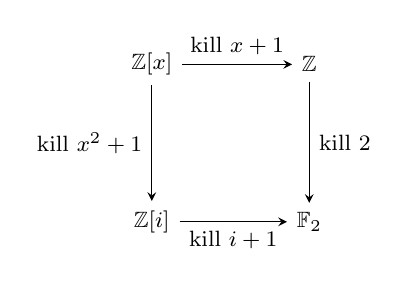
\begin{tikzpicture}[>=stealth, node distance=2cm, font=\footnotesize]
		% Nodes
		\node (Zx) {$\mathbb{Z}[x]$};
		\node[right of=Zx] (Z) {$\mathbb{Z}$};
		\node[below of=Zx] (Zi) {$\mathbb{Z}[i]$};
		\node[below of=Z] (F2) {$\mathbb{F}_2$};
		
		% Arrows
		\draw[->] (Zx) -- (Z) node[midway, above] {kill $x+1$};
		\draw[->] (Zx) -- (Zi) node[midway, left] {kill $x^2+1$};
		\draw[->] (Z) -- (F2) node[midway, right] {kill $2$};
		\draw[->] (Zi) -- (F2) node[midway, below] {kill $i+1$};
	  
	  \end{tikzpicture}
\end{center}

\newpage
\section*{Problem 5}
\begin{enumerate}[(a)]
	\item The ring $\mathbb{Z}/n\mathbb{Z}$ has characteristic $n$.
	\item We have that $n\cdot a = n\cdot (1 \cdot a) = (n\cdot 1) \cdot a = 0$.
\end{enumerate}
\newpage 

\section*{Problem 6}
Over the integers, Pascal's identity says
\begin{align*}
	\binom{n}{i-1} + \binom{n}{i} &=\frac{n!}{(i-1)!(n+1-i)!}+\frac{n!}{i!(n-i)!} \\
	&= n!\left(\frac{i}{i!(n+1-i)!}+\frac{n+1-i}{i!(n+1-i)!}\right) \\
	&= n!\left(\frac{n+1}{i!(n+1-i)!}\right) \\ 
	&= \frac{(n+1)!}{i!(n+1-i)!} \\ 
	&= \binom{n+1}{i}.
\end{align*}
We can prove the binomial theorem by induction.
In the base case where $n=1$ then
\[
	(a+b) = a^0b^1 + a^1b^0
\]
Assuming that the binomial theorem holds for $n$,
we will now prove it holds for $n+1$
using the distributive property for rings and Pascal's identity for integers.
\begin{align*}
	(a+b)^{n+1} &= (a+b)(a+b)^n \\
	&= (a+b)\sum_{i=0}^{n} \binom{n}{i} a^i b^{n-i} \\
	&= \sum_{i=0}^{n} \binom{n}{i} a^{i+1} b^{n-i} + \sum_{i=0}^{n} \binom{n}{i} a^i b^{n+1-i} \\
	&= \sum_{i=1}^{n+1} \binom{n}{i-1} a^{i} b^{n+1-i} + \sum_{i=0}^{n} \binom{n}{i} a^i b^{n+1-i} \\
	&= \sum_{i=0}^{n+1} \binom{n}{i-1} a^{i} b^{n+1-i} + \sum_{i=0}^{n+1} \binom{n}{i} a^i b^{n+1-i} \\
	&= \sum_{i=0}^{n+1} \left( \binom{n}{i-1} +\binom{n}{i}\right)a^{i} b^{n+1-i}\\
	&= \sum_{i=0}^{n+1} \binom{n+1}{i} a^{i} b^{n+1-i}
\end{align*}

Notice that we rewrote the range of summation for convenience 
since the terms where $i=0$ and $i=n+1$ are equal to zero.
\newpage 

\section*{Problem 7}
The homomorphism sends $1$ to $1$.
\[
	\phi(1) = 1^p = 1.
\]
The homomorphism respects multiplication
\[
	\phi(ab) = (ab)^p = a^pb^p = \phi(a)\phi(b)
\]
Notice that 
\[
	\binom{p}{i} = \frac{p!}{i!(p-i)!}
\]
is a multiple of $p$ for $0<i<p$
since $i!$ and $(p-i)!$ are coprime with $p$ when $p$ is prime.

Using the binomial theorem, the homomorphism respects addition.
\begin{align*}
	\phi(a+b) &= (a+b)^p \\
	 &= \sum_{i=0}^{p} \binom{p}{i} a^i b^{p-i} \\
	 &= a^p + b^p \\
	 &= \phi(a) + \phi(b)
\end{align*}


















\end{document}